\documentclass[tikz,crop]{standalone}
\usepackage{amsmath}
\usepackage{amssymb}
\usepackage[english]{babel}
\usepackage[utf8]{inputenc}
\usepackage[T1]{fontenc}
\usepackage{euler}

\usepackage{tikz}
\usetikzlibrary{matrix, shapes, arrows, positioning}

\begin{document}

	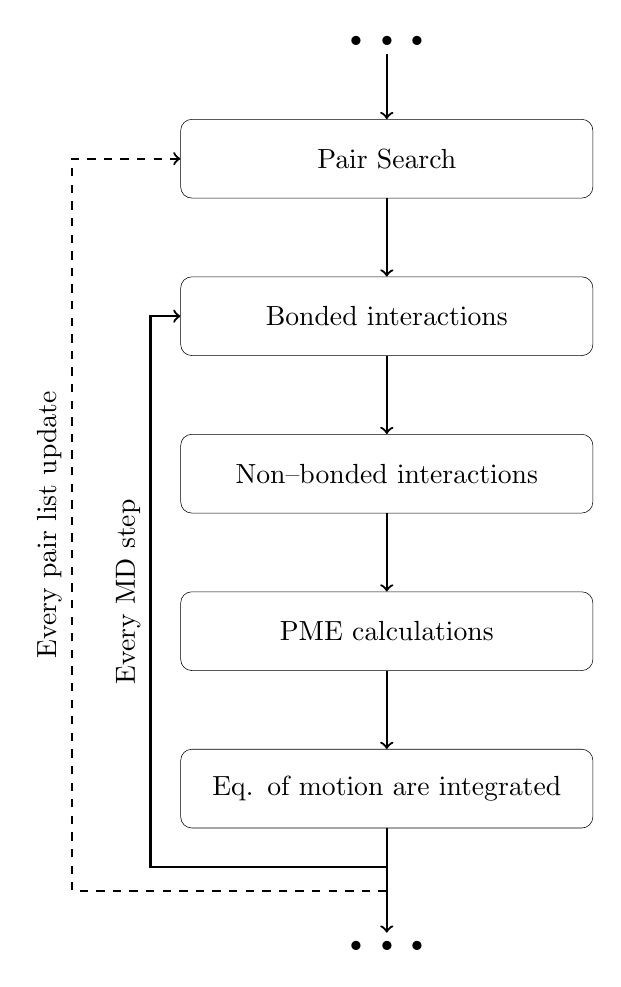
\begin{tikzpicture}
		%\draw[gray,step=1] (-7,0) grid (7,15);
		\node[align=center] (0) at (0,11.5) {\Huge$\ldots$};
		\node[rectangle,draw,rounded corners,very thin,minimum width=5cm,minimum height=1cm,text width=5cm,align=center] (A) at (0,10) {Pair Search};
		\node[rectangle,draw,rounded corners,very thin,minimum width=5cm,minimum height=1cm,text width=5cm,align=center] (B)  at (0,8) {Bonded interactions};
		\node[rectangle,draw,rounded corners,very thin,minimum width=5cm,minimum height=1cm,text width=5cm,align=center] (C)  at (0,6) {Non--bonded interactions};
		\node[rectangle,draw,rounded corners,very thin,minimum width=5cm,minimum height=1cm,text width=5cm,align=center] (D)  at (0,4) {PME calculations};
		\node[rectangle,draw,rounded corners,very thin,minimum width=5cm,minimum height=1cm,text width=5cm,align=center] (E)  at (0,2) {Eq. of motion are integrated};
		\node[align=center] (F) at (0,0) {\Huge$\ldots$};

		\node (F1) at (0,1) {};
		\node (F2) at (0,0.7) {};

		\draw[thick,->] (0) -- (A);
		\draw[thick,->] (A) -- (B);
		\draw[thick,->] (B) -- (C);
		\draw[thick,->] (C) -- (D);
		\draw[thick,->] (D) -- (E);
		\draw[thick,->] (E) -- (F);

		\draw[thick, ->] (F1.center) -- (-3,1) -- (-3,8) node[midway, above, rotate=90] {Every MD step} |- (B);
		\draw[thick,dashed,->] (F2.center) -- (-4, 0.7) -- (-4, 10) node[midway, above, rotate=90] {Every pair list update} |- (A);

	\end{tikzpicture}

\end{document}
	